\AtBeginSection[]{
    \begin{frame}
        \frametitle{}
        \tableofcontents[currentsection]
    \end{frame}
}

%%%%%%%%%%%%%%%%%%%%%%%%%%%%%%%%%%%%

\section{Evaluation in cooperative game environments}

\begin{frame}{Evaluation in cooperative game environments}

    \begin{block}{Atari-like environments}
        \begin{itemize}
            \item \textquote{Drone swarm - 3rd CAGE Challenge}~\cite{cage_challenge_3_announcement} (CYB);
            \item \textquote{Pistonball} (PBL)~\cite{Terry2021};
            \item \textquote{Predator-prey with communication}~\cite{Lowe2017} (PPY);
            \item \textquote{Knights Archers Zombies}~\cite{Terry2021}.
        \end{itemize}

        \begin{figure}[H]
            \centering
            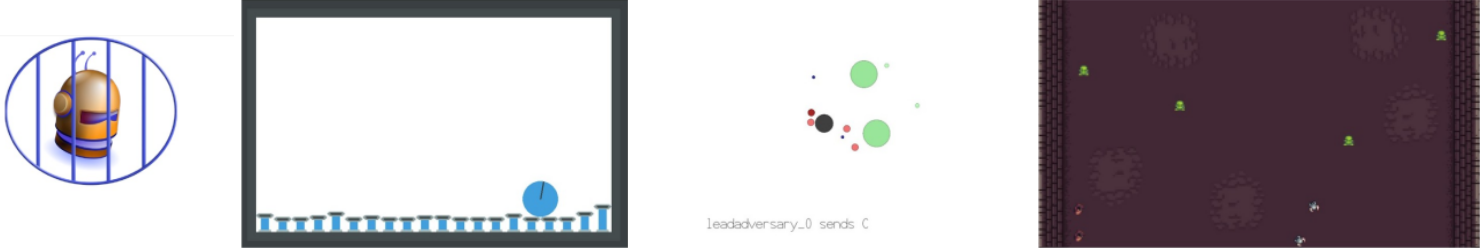
\includegraphics[width=0.5\linewidth]{figures/envs_4x1.png}
            \caption{Overview of the selected environments: CYB, PBL, PPY, and KAZ}
            \label{fig:simulated_environments}
        \end{figure}

    \end{block}

    \begin{block}{Application modes of AOMEA}
        \begin{itemize}
            \item No organizational specifications (NTS)
            \item Partially constraining organizational specifications (PTS)
            \item Fully constraining organizational specifications (FTS)
        \end{itemize}
    \end{block}

\end{frame}

\begin{frame}[allowframebreaks]{Evaluation in cooperative game environments}{Results on training performance}

    \begin{columns}

        \begin{column}{0.3\textwidth}
            { \tiny
                \begin{table}[t!]

    \centering

    \begin{tblr}{colspec={llll},rows={m},measure=vbox,stretch=-1}

        \textbf{Environment} & \textbf{PTS/NTS} & \textbf{PTS/FTS} & \textbf{Perf. stability \\ (avg. / max)} \\

        \hline

        { PPL }
        & { 4.7 }
        & { 1.3 }
        & { 0.9 } \\

        \hline[dashed]

        { PPY }
        & { 6.3 }
        & { 2.2 }
        & { 0.78 } \\

        \hline[dashed]

        { KAZ }
        & { 4.0 }
        & { 1.1 }
        & { 0.42 } \\

        \hline[dashed]

        { CYB }
        & { 12 }
        & { 3.3 }
        & { 0.36 } \\


    \end{tblr}

    \caption{View of the AOMEA approach impact during training}

    \label{tab:training_AOMEA_results}

\end{table}
}

        \end{column}

        \hspace{1ex}

        \begin{column}{0.7\textwidth}
            \begin{figure}[h!]
                \centering
                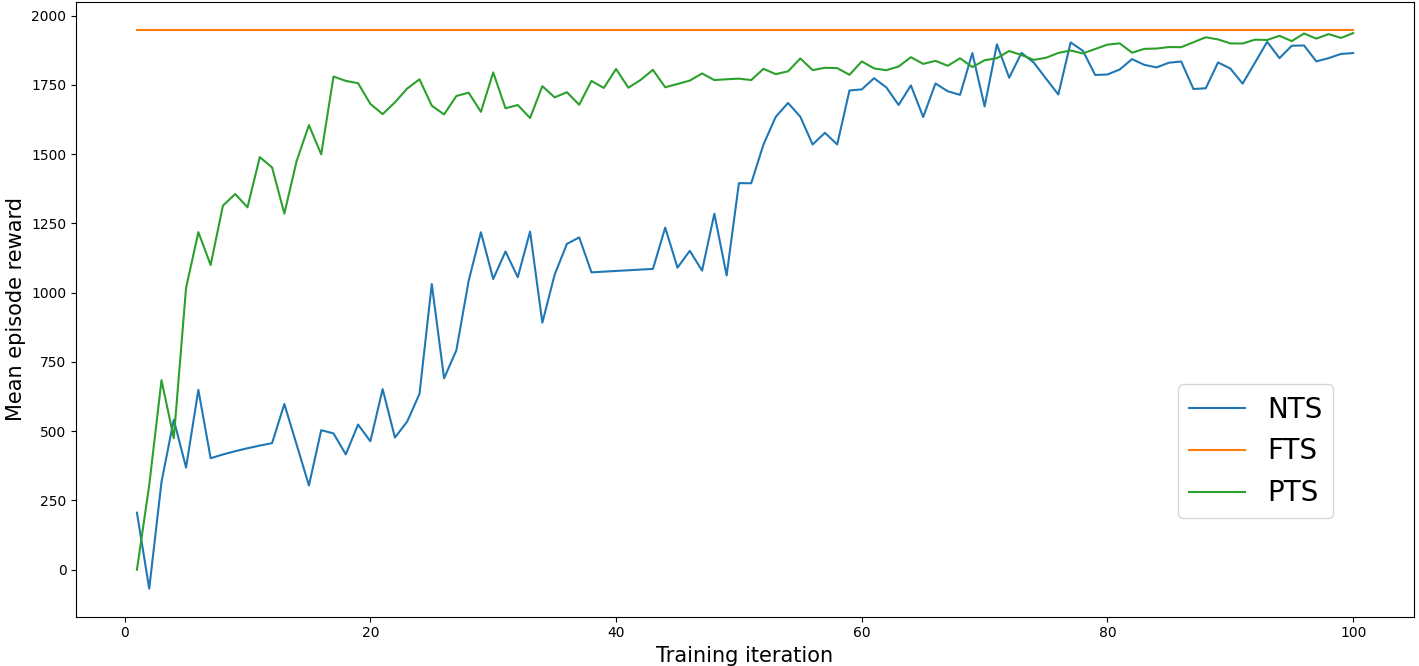
\includegraphics[width=0.95\textwidth]{figures/prahom_learning_curve.png}
                \caption{Average reward for each iteration in the PBL environment for the NTS, PTS, and FTS cases}
                \label{fig:prahom_learning_curve}
            \end{figure}
        \end{column}

    \end{columns}

    \begin{block}{Analysis}

        \begin{itemize}
            \item \textbf{search space decreasing}: convergence time is longer for NTS than for PTS which is also longer than for FTS;
            \item \textbf{NTS outperformance}: trained agents' policies are hand-tailored to solve the problem much more finely than the designer's organizational specifications;
            \item \textbf{Impact on solving strategy}: low-performance stability in CYB environment $\rightarrow$ no general strategies compared to the other environments.
        \end{itemize}

    \end{block}

\end{frame}

\begin{frame}[allowframebreaks]{Evaluation in cooperative game environments}{Performance results after training}

    \begin{columns}

        \begin{column}{0.3\textwidth}
            { \tiny
                \begin{table}[t!]

    \centering

    \begin{tblr}{colspec={llll},rows={m},measure=vbox,stretch=-1}

        \textbf{Environment} & \textbf{Roles} & \textbf{Links} & \textbf{Global performance} \\

        \hline

        { 1 }
        & {  }
        & {  } \\
        & {  } \\

        \hline[dashed]

        { 2 }
        & {  }
        & {  } \\
        & {  } \\

        \hline[dashed]

        { 3 }
        & {  }
        & {  } \\
        & {  } \\

        \hline[dashed]

        { 4 }
        & {  }
        & {  } \\
        & {  } \\

        \hline[dashed]

        { 5 }
        & {  }
        & {  } \\
        & {  } \\

    \end{tblr}

    \caption{View of the OOMARL approach impact after training}

    \label{tab:trained_OOMARL_results}

\end{table}

            }

        \end{column}

        \hspace{1ex}

        \begin{column}{0.7\textwidth}
            \begin{figure}[h!]
                \centering
                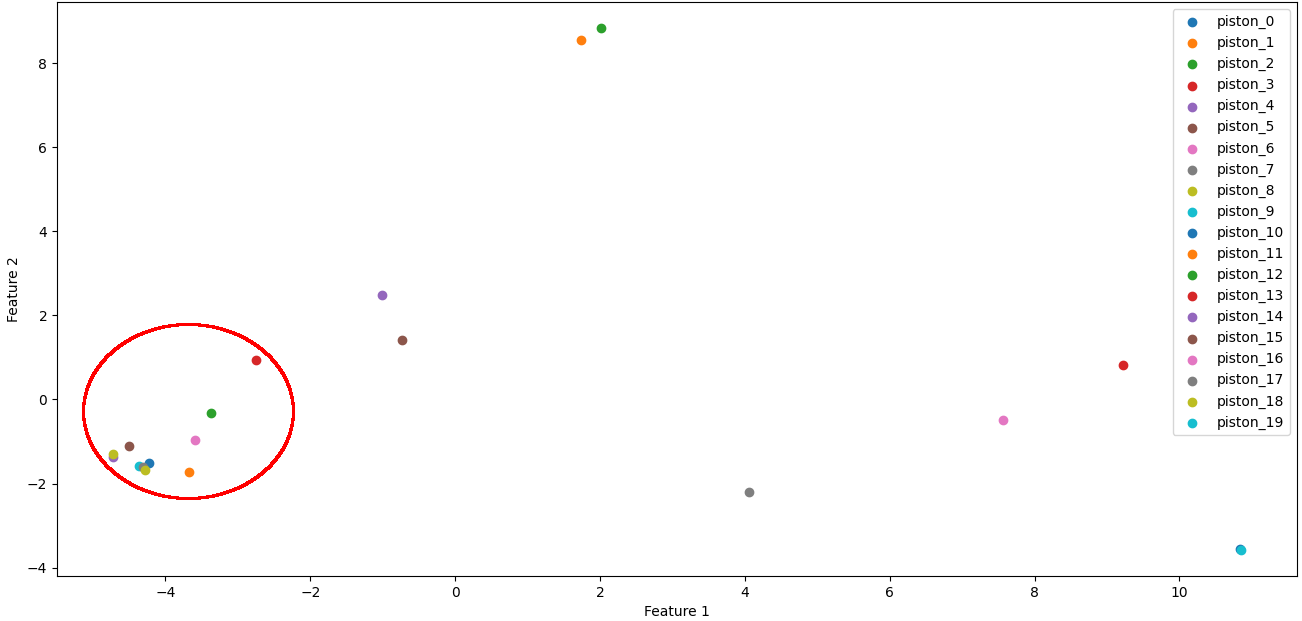
\includegraphics[width=\textwidth]{figures/prahom_pca_analysis.png}
                \caption{PCA of the trained agents' histories in the PBL environment}
                \label{fig:prahom_pca_analysis}
            \end{figure}
        \end{column}

    \end{columns}

    \begin{block}{Analysis}
        \begin{itemize}
            \item \textbf{PBL}: most agents’ histories are in the left bottom zone of the PCA $\rightarrow$ share a common role;
            \item \textbf{KAZ}: archers tend to move away from zombies, while knights tend to approach them $\rightarrow$ two roles;
            \item \textbf{PPY}: authority links between the leader predator and the simple predators $\rightarrow$ collective strategies for circling prey
            \item \textbf{CYB}: communication links $\rightarrow$ isolate infiltrated drones or trying to fix and alert recently suspected drones.
        \end{itemize}
    \end{block}

\end{frame}
